\documentclass[a4paper,11pt,final]{article}

\usepackage[utf8]{inputenc} 
\usepackage[T1]{fontenc}


\usepackage{lmodern}

\usepackage{graphicx}
\graphicspath{{../book-result/Slides/4-Done/}{../book-result/Slides/figures/}}


\usepackage{tikz}

\usepackage{calc}

\usepackage{xspace}

\usepackage[absolute,overlay]{textpos} 

\usepackage{url}

\usepackage[unicode]{hyperref}

\hypersetup{
	colorlinks,
	menucolor=black,
	urlcolor=black,
	linkcolor=black,
	pdftitle={Pharo MOOC}, 
    pdfauthor={Damien Cassou, Stéphane Ducasse and Luc Fabresse}
}

\setlength{\pdfpagewidth}{210mm} 
\setlength{\pdfpageheight}{297mm}
\usepackage[a4paper,pdftex,twoside,nomarginpar,inner=20mm,outer=20mm,top=20mm,bottom=20mm]{geometry}

\usepackage[final]{pdfpages}

%
% Boxed environment with semi-transparent shadow.
% http://www.texample.net/tikz/examples/transparent-shadows/
\newlength{\boxw}
\newlength{\boxh}
\newlength{\shadowsize}
\newlength{\boxroundness}
\newlength{\tmpa}
\newsavebox{\shadowblockbox}

\setlength{\shadowsize}{6pt}
\setlength{\boxroundness}{3pt}

\newenvironment{shadowblock}[1]%
{\begin{lrbox}{\shadowblockbox}\begin{minipage}{#1}}%
{\end{minipage}\end{lrbox}%
\settowidth{\boxw}{\usebox{\shadowblockbox}}%
\settodepth{\tmpa}{\usebox{\shadowblockbox}}%
\settoheight{\boxh}{\usebox{\shadowblockbox}}%
\addtolength{\boxh}{\tmpa}%
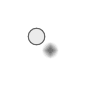
\begin{tikzpicture}
    \addtolength{\boxw}{\boxroundness * 2}
    \addtolength{\boxh}{\boxroundness * 2}

    \foreach \x in {0,.05,...,1}
    {
        \setlength{\tmpa}{\shadowsize * \real{\x}}
        \fill[xshift=\shadowsize - 1pt,yshift=-\shadowsize + 1pt,
                black,opacity=.04,rounded corners=\boxroundness]
            (\tmpa, \tmpa) rectangle +(\boxw - \tmpa - \tmpa,
                \boxh - \tmpa - \tmpa);
    }

    \filldraw[fill=black!08, draw=black!60, rounded corners=\boxroundness]
        (0, 0) rectangle (\boxw, \boxh);
    \draw node[xshift=\boxroundness,yshift=\boxroundness,
        inner sep=0pt,outer sep=0pt,anchor=south west]
             (0,0) {\usebox{\shadowblockbox}};
\end{tikzpicture}}




\begin{document}

\thispagestyle{empty}
\begin{center}
	\vspace*{1em}

	~\vfill %%%
	
	\begin{shadowblock}{\linewidth}
		\centering
		\begin{minipage}{\linewidth}
		\noindent\vspace*{1em}
		\begin{center}
		\textbf{\Huge Pharo MOOC}
		
		\vspace*{3.5em}
	
		{\LARGE Damien Cassou, Stéphane Ducasse and Luc Fabresse}
      
      \vspace*{2em}
      
      2015\\  
      \vspace*{0.5em}
	\end{center}    
	 
      \vspace*{1em}
	\end{minipage}
	\end{shadowblock}
\end{center}

~\vfill %%%

\clearpage

% =======================
% Week1
% =======================
% \markboth{}
% \phantomsection%
% \addcontentsline{toc}{section}{Dossier d'inscription en HDR}
% \label{sec:formulaireInsc}
% \includepdf[pages={-}]{}

\includepdf[pages={-}]{AdvancedDidYouReallyUnderstandSuper-2x4.pdf}
\includepdf[pages={-}]{Basic-ArraySetOrderedCollection-2x4.pdf}
\includepdf[pages={-}]{Basic-BooleansAndCondition-2x4.pdf}
\includepdf[pages={-}]{Basic-ClassAndMethodDefinition-2x4.pdf}
\includepdf[pages={-}]{Basic-ClassMethods-2x4.pdf}
\includepdf[pages={-}]{Basic-ClassMethodsAtWork-2x4.pdf}
\includepdf[pages={-}]{Basic-Exceptions-2x4.pdf}
\includepdf[pages={-}]{Basic-Loops-2x4.pdf}
\includepdf[pages={-}]{Basic-Numbers-2x4.pdf}
\includepdf[pages={-}]{Basic-RuntimeArchitecture-2x4.pdf}
\includepdf[pages={-}]{Basic-Streams-2x4.pdf}
\includepdf[pages={-}]{Basic-Variables-2x4.pdf}
\includepdf[pages={-}]{Blocks-2x4.pdf}
\includepdf[pages={-}]{Blocks-Loops-2x4.pdf}
\includepdf[pages={-}]{Design-AboutFinalAndOthers-2x4.pdf}
\includepdf[pages={-}]{Design-AvoidIsNil-2x4.pdf}
\includepdf[pages={-}]{Design-ClassAsObjects-2x4.pdf}
\includepdf[pages={-}]{Design-EssenceOfDispatch-2x4.pdf}
\includepdf[pages={-}]{Design-EssenceOfDispatchExo-2x4.pdf}
\includepdf[pages={-}]{Design-HookAndTemplate-2x4.pdf}
\includepdf[pages={-}]{Design-HooksAndTemplate-2x4.pdf}
\includepdf[pages={-}]{Design-LibrariesVsFrameworks-2x4.pdf}
\includepdf[pages={-}]{Design-SelfSendsArePlanForReuse-2x4.pdf}
\includepdf[pages={-}]{Design-WhyTesting-2x4.pdf}
\includepdf[pages={-}]{InheritanceAndLookup-1-Inheritance-2x4.pdf}
\includepdf[pages={-}]{InheritanceAndLookup-2-Lookup-2x4.pdf}
\includepdf[pages={-}]{InheritanceAndLookup-3-Super-2x4.pdf}
\includepdf[pages={-}]{InheritanceAndLookup-4-DoesNotUnderstand-2x4.pdf}
\includepdf[pages={-}]{InheritanceAndLookup-5-LookupMetaclasses-2x4.pdf}
\includepdf[pages={-}]{Intro-ModelInaNushell-2x4.pdf}
\includepdf[pages={-}]{Intro-SyntaxInANutshell-2x4.pdf}
\includepdf[pages={-}]{Intro-SyntaxInANutshell-newVersion-2x4.pdf}
\includepdf[pages={-}]{Iterators-2x4.pdf}
\includepdf[pages={-}]{Message-ParenthesisVsSquareBrackets-2x4.pdf}
\includepdf[pages={-}]{Messages-2x4.pdf}
\includepdf[pages={-}]{Messages-ForTheJavaProgrammers-2x4.pdf}
\includepdf[pages={-}]{Messages-Precedence-2x4.pdf}
\includepdf[pages={-}]{Messages-Sequence-2x4.pdf}
\includepdf[pages={-}]{ObjectivesCourse-2x4.pdf}
\includepdf[pages={-}]{ObjectivesMooc-2x4.pdf}
\includepdf[pages={-}]{TeapotServer-2x4.pdf}
\includepdf[pages={-}]{TestAdvocado-2x4.pdf}


\end{document}

  
